\documentclass[a4paper]{article}

\usepackage{cite}%多个文献引用
\usepackage{graphicx}
\usepackage{array}%调节表格行高
\usepackage{multirow,makecell}%多行表格
\usepackage{tabularx}%表格固定列宽
\usepackage{subfigure}
\usepackage{titlesec}%标题格式设置
\usepackage{amsmath}
\usepackage{amssymb}
\usepackage{tabularx}
\usepackage{makecell}
\usepackage{geometry}
\usepackage{float}
\usepackage{setspace}%行距包
\usepackage{siunitx}
\usepackage{mdwlist}
\usepackage{tabu}
\usepackage{enumerate}

\geometry{top=1.54cm,bottom=2.54cm,left=2.5cm,right=2.5cm}


\begin{document}
\begin{center}
\bf\Large
EE 105 Feedback Control Systems\par
Department of Electrical and Computer Engineering\par
Tufts University Fall 2018\par
Homework \#5\par   
\end{center}
\begin{table}[H]
\begin{center}
\begin{tabular*}{\textwidth}{@{\extracolsep{\fill}}lcr}
Name: {\it Shang Wang} &Student ID: {\it 1277417} &E-mail: {\it shang.wang@tufts.edu}\\
\hline
\end{tabular*}
\end{center}
\end{table}

\section{Problem 1}
\subsection{Part A} 
$$L(s) = \frac{(s+2)(s+6)}{s(s+1)(s+5)(s+10)}$$
{\bf Answer:}\\
Poles at ($p = 0, -1, -5, -10$), while zeros at ($z = -2, -6$). All the poles and zeros are in the real axis. So the pole(p = -10) will finally find ($z = -6$), likewise, ($p = -5$) will reach the point ($z = -2$). The other two poles ($p = 0$) and ($p = -1$) will join together, then seperat with departure angle $\pm \theta_d$, finally go to infinity with angle $\pm \pi/2$. The remaining parameters depature angle $\theta_d$, Real-Axis intercept $\alpha$ and Break Away point $\sigma$ still need to be calculated.\\
\\
The "Real-Axis intercept" $\alpha$:
$$
\alpha = \frac{\sum_{1}^{n}p_i-\sum_1^m z_j}{n-m} = -4
$$
The "Break Away point" $\sigma$ (which is a real number) satisfies the formular:
$$
\frac{\rm d}{{\rm d}\sigma}K  = \frac{{\rm d}}{{\rm d}\sigma}\frac {-1} {L(\sigma)} = 0
$$
Meaning :
$$
\frac{\rm d}{{\rm d}\sigma}\frac{-\sigma(\sigma+1)(\sigma+5)(\sigma+10)}{(\sigma+2)(\sigma+6)} = 0
$$
We have $\sigma$:
$$
\sigma = -0.5676
$$
Then we can calculate the departure angle $\theta_d$. Assume $s_0 = b+xi$ is on the root locus near break away point. The angle is really small so we have $\tan(\theta) = \theta$. Using Master Criterian.
$$
\sum_{i=1}^n \frac{x}{b - z_i} - \sum_{j=1}^m \frac{x}{b - p_j} = \pm\pi
$$
$$
x\cdot f(b) = \pm\pi\rightarrow \frac{x}{b-\sigma} = \tan(\theta_d) = \pm \frac{\pi}{f(b)(b - \sigma)}
$$
Where $f(b) = \sum_{i=1}^n \frac{1}{b - z_i} - \sum_{j=1}^m \frac{1}{b - p_j}$, clearly $\sigma \neq z_i,p_j$. Thus we have:
$$
\lim_{b\rightarrow\sigma}f(b) = \rm Const
$$
So, 
$$
\lim_{b\rightarrow\sigma}\tan(\theta_d) = \pm\infty
$$
We have $\theta_d = \pm\pi/2$.\\
The plot is like:
\begin{figure}[H]
\centering
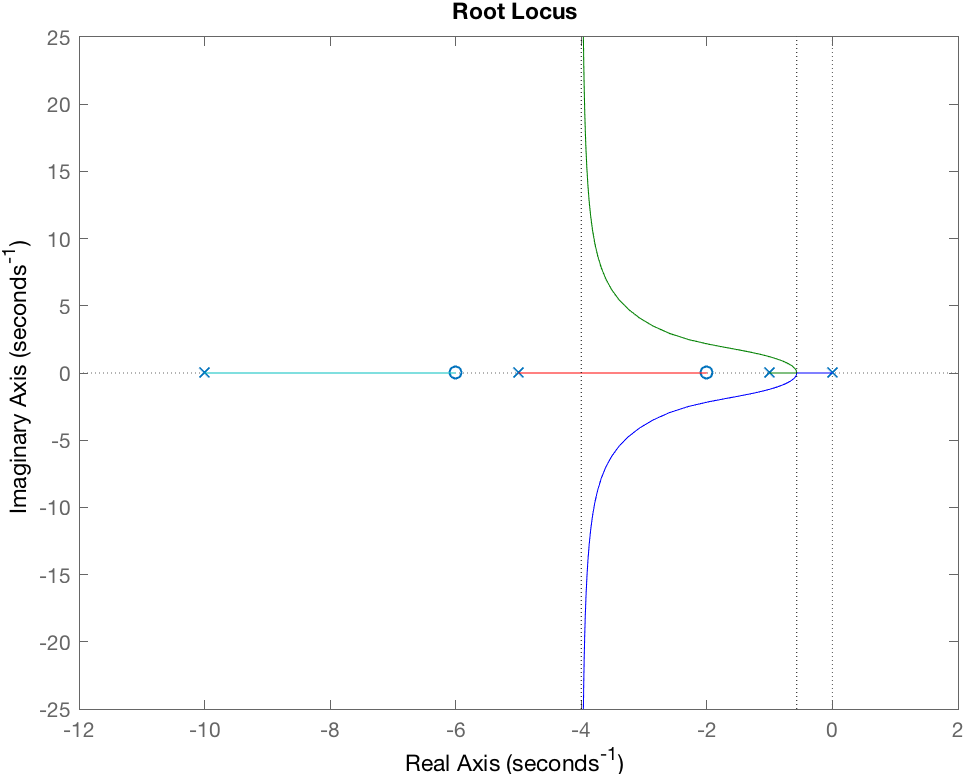
\includegraphics[width = 0.6\textwidth]{pic/t1.png}
\end{figure}

\subsection{Part B}
$$
L(s) = \frac{s^2+2s+12}{s(s^2+2s+10)}
$$
{\bf Answer:}\\
Poles at ($p = 0, -1\pm 3i$), zeros at ($z = -1\pm i\sqrt{11}$). Poles ($p =  -1\pm 3i$) will finally find zeros $z = -1\pm i\sqrt{11}$. Pole $p = 0$ will go to minus infinity on the real axis. \\
\\
The Real-Axis intercept $\alpha$:
$$
\alpha = \frac{\sum_{1}^{n}p_i-\sum_1^m z_j}{n-m} = 0
$$
The departure angle of pole($p = -1+3i$) is $\theta_d$
$$
-\theta_d +  \sum\psi_i-\sum \phi_j = - \pi
$$
We have:
$$
-\theta_d -\pi/2 - (\pi - \arctan(\frac{3}{1})) = -\pi
$$
$$
\theta_d = \arctan(3) - \pi/2 = -18.44^{\circ} 
$$
The departure angle of pole($p = -1-3i$) is $\theta_d = 18.44^{\circ}$.\\
So the plot is:
\begin{figure}[H]
\centering
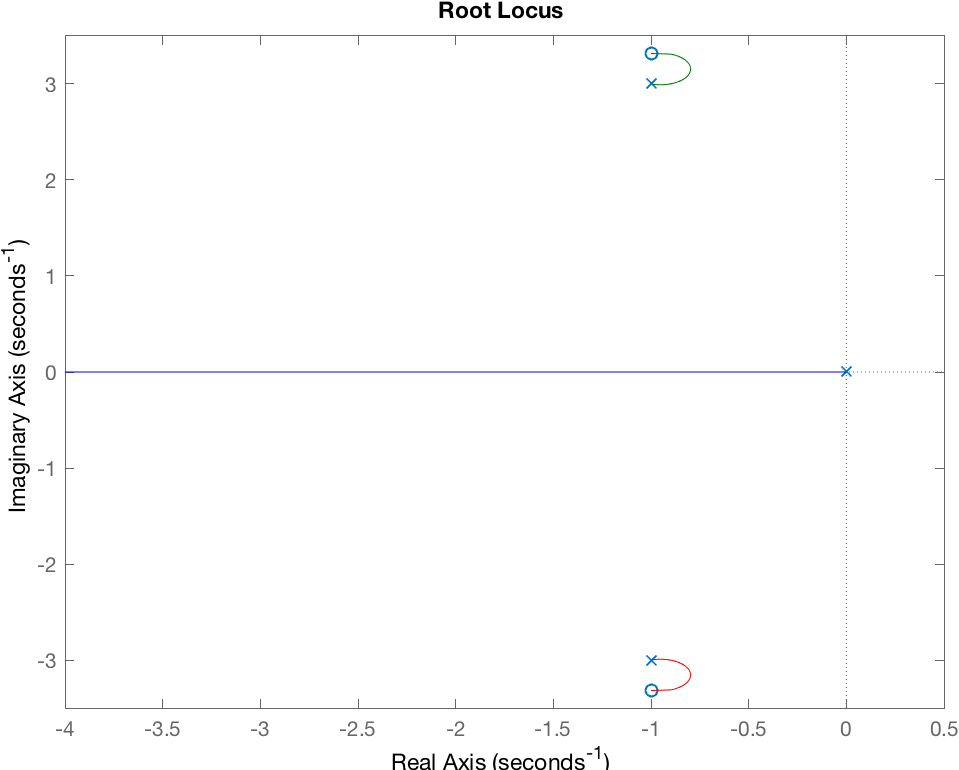
\includegraphics[width = 0.6\textwidth]{pic/t2.png}
\end{figure}

\subsection{Part C}
$$
L(s) = \frac{s+3}{s^3(s+4)}
$$
{\bf Answer:}\\
Poles at ($p = -4$), triple poles at $p = 0$, zeros at $z = -3$. One of the triple poles will find the zero($z = -3$), the other two will flee to infinity. Pole($p = -4$) will go to minus infinity. The departure angle of two poles at ($p = 0$) $\theta$ are:
$$
-3\theta_d +  \sum\psi_i-\sum \phi_j = \pm \pi
$$
We have $\theta_d = \pm \pi/3$.\\
The real axis intercept $\alpha$:
$$
\alpha = \frac{\sum_{1}^{n}p_i-\sum_1^m z_j}{n-m} = -\frac14
$$
The Asymptote Angles at Large $s$, we have:
$$
\angle\frac{1}{s^3} = (2n+1)\pi,\ n \in \mathbb{Z}
$$
So the asymptote angle $\theta_a$:
$$
\theta_a = \pm\frac{\pi}{3},\pi
$$
The plot is like this:
\begin{figure}[H]
\centering
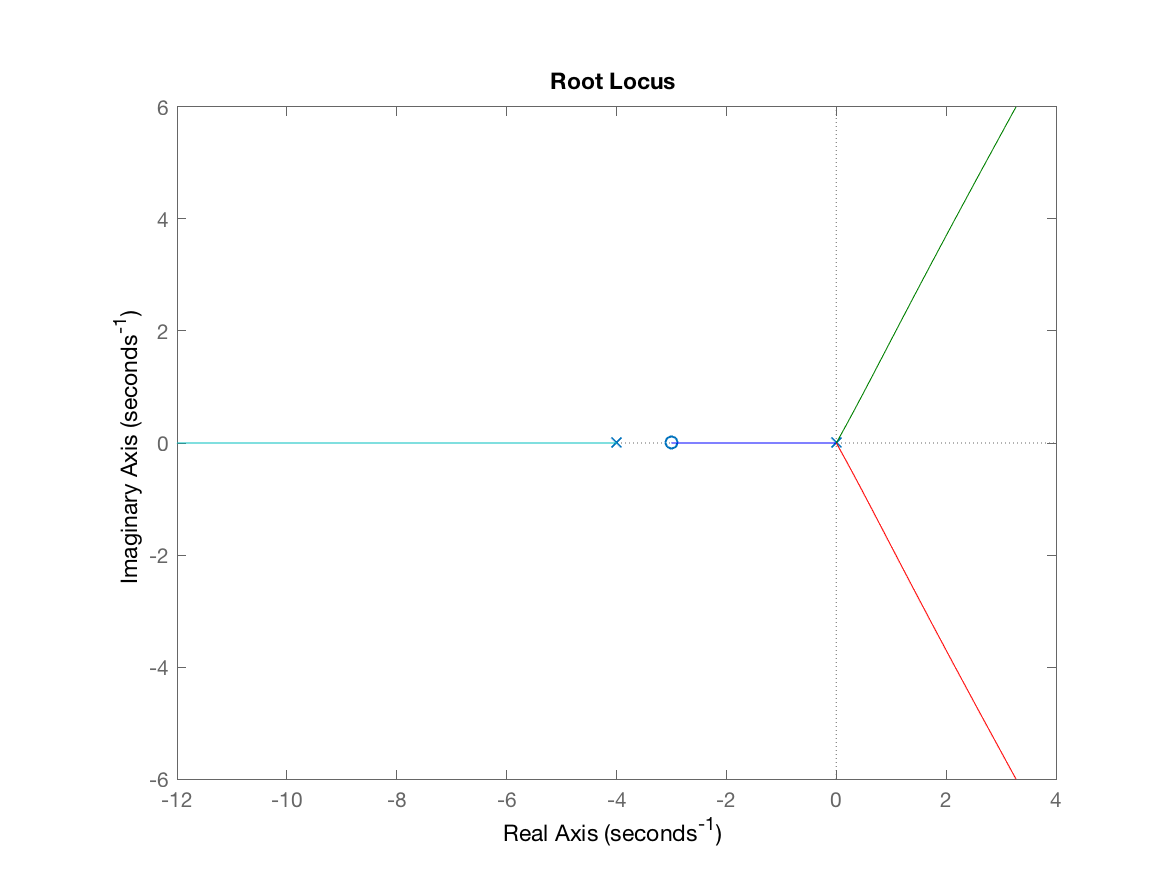
\includegraphics[width = 0.6\textwidth]{pic/t3.png}
\end{figure}


\section{Problem 2}
\subsection{Part A}
{\bf Answer:}\\
$G(s)$ has poles at ($p = 0,1$), no zeros. So the two poles will join together and break away to infinity at $\sigma = 1/2$ on the real axis. Their departure angle and asymptote angle are both $\pm \pi/2$. Thus, it's impossible for the root locus to have interception with imaginary axis $Re(s) = -1$ at $s = -1 \pm j\sqrt{3}$. \\

\noindent The root locus is like this:
\begin{figure}[H]
\centering
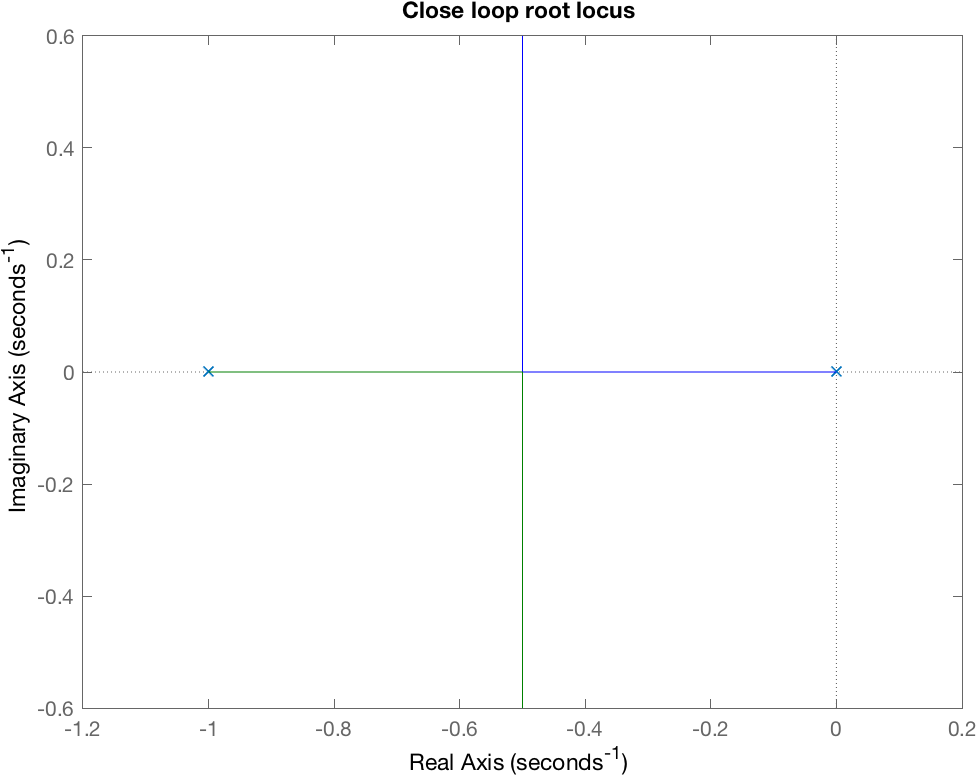
\includegraphics[width = 0.6\textwidth]{pic/t4.png}
\end{figure}
\subsection{Part B}
{\bf Answer:}\\
Write the close loop transfer function:
$$
H(s) = \frac{D_c(s)G(s)}{1+D_c(s)G(s)} = \frac{K(s+z)}{s^3+(1+p)s^2+(p+K)s+z}
$$
According to the requirement, we need close loop poles at $p = -1\pm i\sqrt{3}$. So, we can write a denominator:
$$
(s^2 + 2s + 4)(s+2) = s^3 + 4s^2 + 8s + 8
$$
Parameter $K,p,m$ can be calculated accordingly.
$$
p = 3, \ K = 5,\ z = \frac85
$$
Thus, 
$$
D_c(s) = \frac{4(s+8/5)}{s+3}
$$
The root locus plot is like:
\begin{figure}[H]
\centering
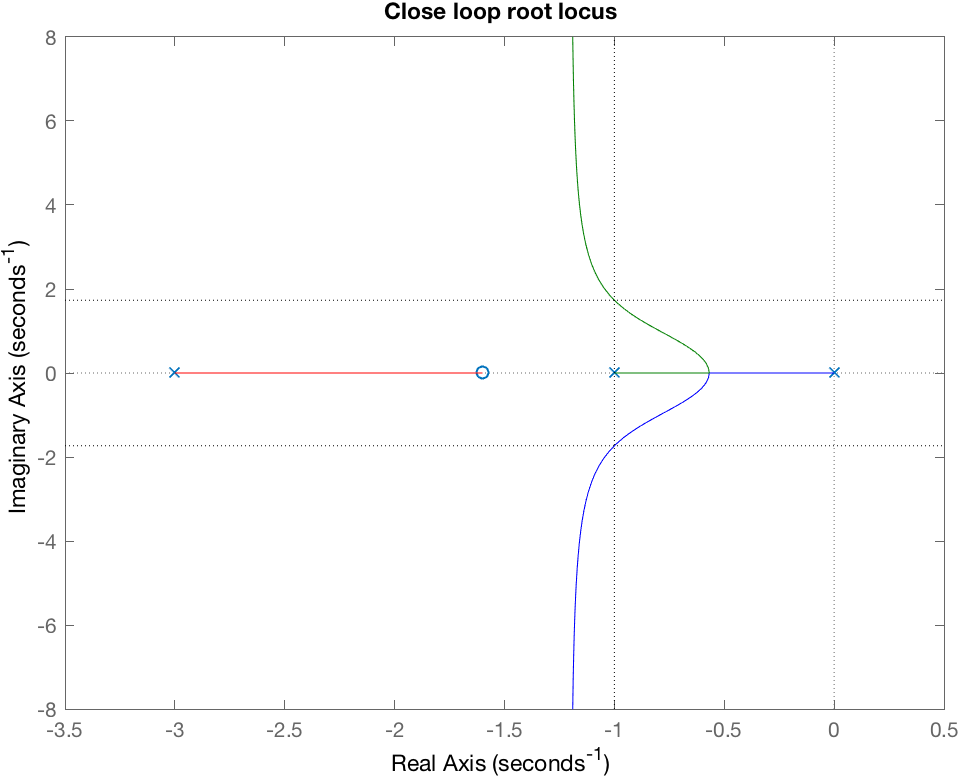
\includegraphics[width = 0.6\textwidth]{pic/t5.png}
\end{figure}







\end{document}